\section{Evaluation}
\label{sec:eval}
\subsection{Methodology}

\textbf{Evaluation Models and Datasets.}
We evaluate \proj using three representative VLMs with video understanding and reasoning capabilities: Llava-OneVision-7B (Llava-OV)~\cite{li2024llava}, Llava-Video-7B (Llava-Vid)\cite{zhang2024video}, and MiniCPMV-2.6 (MiniCPM)~\cite{yao2024minicpm}. These models are tested on three widely adopted video understanding benchmarks: VideoMME (VMME)~\cite{fu2025video}, MVBench (MVB)~\cite{li2024mvbench}, and MLVU~\cite{zhou2025mlvu}. These datasets include diverse video types and durations, enabling a holistic evaluation of model capabilities across comprehension, temporal reasoning, and multimodal alignment.
We use open-source models obtained from HuggingFace Transformers~\cite{wolf2020transformers} and perform evaluation via the \texttt{lmms-eval}~\cite{zhang2024lmmsevalrealitycheckevaluation} multimodal benchmarking framework to ensure consistency and fairness.

\textbf{Baselines.}
We compare \proj against two state-of-the-art architectures: AdapTiV~\cite{yoo2024adaptiv}, a vision transformer accelerator, and CMC~\cite{song2024cmc}, an accelerator optimized for video transformers. We extend their designs to make them compatible with VLMs. {CMC performs inter-frame similarity checks, whereas AdapTiV focuses on intra-frame similarity detection; both exclude text tokens.} We also compare with the vanilla systolic array~\cite{kung1979systolic} architecture for a base reference.
In addition to hardware baselines, we also compare with FrameFusion~\cite{fu2024framefusion}, a state-of-the-art token pruning algorithm tailored for efficient VLMs with video inputs. 

\begin{table}[b]
% \vspace{-7mm}
    \centering
    \caption{{\proj Architecture Setup}}
    \resizebox{0.5\textwidth}{!}{
    \begin{tabular}{l|l}
    \toprule
        PE Array & 32 $\times$ 32; FP16 Mul FP32 Acc; Weight Stationary \\ \midrule
        \proj Hyper-params & Block Size: 2$\times$2$\times$2; Vector Length: 32; \\
        & Similarity Threshold: 0.9; M Tile Size: 1024\\
        & {Semantic: Retain 40\%/30\%/20\%/15\%/10\%} \\
        & {of total image tokens at layer 3/6/9/18/26} \\ \midrule
        On-Chip Buffer & Input: 128KB; Weight: 78KB; Output: 512KB; \\
        & Layouter Buffer: 16KB for 256-vector window; \\
        & 734KB in total.
                      \\ \midrule
        Off-Chip Memory & {DDR4 4Gb × 16, 2133R, 4 Channels, 64GB/s} \\ 
    \bottomrule
    \end{tabular}
    }
    \label{tab:hardware-config}
\end{table}
\textbf{Algorithm Implementation of \proj and Baselines.}
We implement the algorithm of our proposed \proj method in PyTorch~\cite{paszke2019pytorch}. For the baselines, we faithfully reproduce the token pruning algorithm from AdapTiV and CMC, carefully tuning their hyperparameters for application to VLMs. For FrameFusion, we adopt the official open-source implementation without modification. All algorithms are executed on an NVIDIA A100 GPU~\cite{nvidia2020a100} using FP16 precision for fair and consistent comparison.

\textbf{Architecture Implementation of \proj and Baselines.}
Our \proj architecture setup is shown in \Tbl{tab:hardware-config}. To evaluate architectural performance, we develop a cycle-accurate simulation framework based on SCALEsim-v2~\cite{samajdar2018scale}. {The simulator accepts layer-wise sparse traces generated from specific models and datasets in our PyTorch implementation, enabling precise modeling of cycles and memory access.} {We implement the \proj architecture in SystemVerilog and generate the on-chip SRAMs using the TSMC N28HPC+ Memory Compiler. The RTL is synthesized with a target clock period of 1.32 ns ($\approx$757 MHz) under the worst-case slow–slow (SS) corner (0.81V, 125°C), achieving 0 ns worst negative slack (WNS) and providing a 34\% timing margin for place-and-route at 500 MHz. The resulting area is reported from post-synthesis analysis, and the on-chip power is obtained from post-synthesis simulation using Synopsys Design Compiler. Off-chip DRAM energy is modeled with DRAMsim3~\cite{li2020dramsim3} for device-level power.}
For a fair comparison, we also implement the core logic of all baseline accelerators in SystemVerilog and evaluate their area and energy using the same toolchain as \proj. 


\begin{table}[t]
    \centering
    \caption{Accuracy and Computation Sparsity of \proj and Baselines}
    \resizebox{0.47\textwidth}{!}{
    \begin{tabular}{l|l|l|c|c|c|c|c}
    \toprule
        Models & Dataset & Metric & Ori. & FF & Ada. & CMC & Ours \\ \midrule
        \multirow{6}{*}{Llava-Vid} 
        & \multirow{2}{*}{VMME} & Acc. & 64.15 & 62.00 & 62.44 & 62.52 & \textbf{62.74} \\ 
        & ~ & Sparsity & 00.00 & 70.00 & 52.15 & 58.62 & \textbf{82.82} \\ \cmidrule{2-8}
        & \multirow{2}{*}{MLVU} & Acc. & 67.74 & 65.38 & 65.94 & 65.17 & \textbf{65.99} \\ 
        & ~ & Sparsity & 00.00 & 70.00 & 32.52 & 42.46 & \textbf{78.26} \\ \cmidrule{2-8}
        & \multirow{2}{*}{MVB} & Acc.  & 60.33 & 57.20 & 57.73 & 58.18 & \textbf{58.20} \\ 
        & ~ & Sparsity & 00.00 & 70.00 & 41.07 & 53.00 & \textbf{78.44} \\ \midrule
        \multirow{6}{*}{Llava-OV} 
        & \multirow{2}{*}{VMME} & Acc. & 58.41 & 57.70 & 58.33 & 58.11 & \textbf{58.70} \\ 
        & ~ & Sparsity & 00.00 & 70.00 & 36.80 & 47.95 & \textbf{81.49} \\ \cmidrule{2-8}
        & \multirow{2}{*}{MLVU} & Acc. & 63.32 & \textbf{62.54} & 62.22 & 62.50 & 62.52 \\ 
        & ~ & Sparsity & 00.00 & 70.00 & 39.55 & 35.48 & \textbf{78.34} \\ \cmidrule{2-8}
        & \multirow{2}{*}{MVB} & Acc.  & 58.38 & \textbf{56.93} & 56.83 & 56.75 & 56.78 \\ 
        & ~ & Sparsity & 00.00 & 70.00 & 42.03 & 63.69 & \textbf{85.49} \\ \midrule
        \multirow{6}{*}{MiniCPM} 
        & \multirow{2}{*}{VMME} & Acc. & 58.81 & \textbf{58.81} & 58.07 & 55.89 & 58.30 \\ 
        & ~ & Sparsity & 00.00 & 70.00 & 49.27 & 57.20 & \textbf{82.87} \\ \cmidrule{2-8}
        & \multirow{2}{*}{MLVU} & Acc. & 55.89 & 54.80 & \textbf{54.84} & 43.80 & 53.59 \\ 
        & ~ & Sparsity & 00.00 & 70.00 & 41.88 & 35.23 & \textbf{78.01} \\ \cmidrule{2-8}
        & \multirow{2}{*}{MVB} & Acc.  & 55.63 & 52.43 & 53.70 & 48.78 & \textbf{54.30} \\ 
        & ~ & Sparsity & 00.00 & 70.00 & 50.09 & 40.27 & \textbf{75.99} \\ 
    \bottomrule
    \end{tabular}
    \label{tab:accuracy}
    }    
% \vspace{-6mm}
\end{table}

\subsection{Algorithmic Accuracy and Theoretical Sparsity}

To evaluate the effectiveness of the multilevel concentration technique in \proj, we compare both model accuracy and the achieved computational sparsity against baseline methods. The computation sparsity is calculated through the ratio of the number of operations using the method to the number of operations required by the systolic array with original input. The results are presented in \Tbl{tab:accuracy}.

\proj consistently achieves the highest accuracy across most evaluated scenarios, outperforming both software-only methods and hardware-based approaches. Compared to the original, uncompressed models, the average accuracy degradation with \proj is only 1.20\%, demonstrating its ability to preserve semantic fidelity.

In addition to maintaining high accuracy, \proj also achieves the highest computational sparsity across all models and datasets. Specifically, \proj achieve sparsity of \textbf{80.19$\%$} on average, delivering 37.37\% and 31.98\% higher sparsity than AdapTiV and CMC, respectively, and outperforms FrameFusion by over 10.19\% in sparsity. 


\begin{figure*}[t]
    \centering
    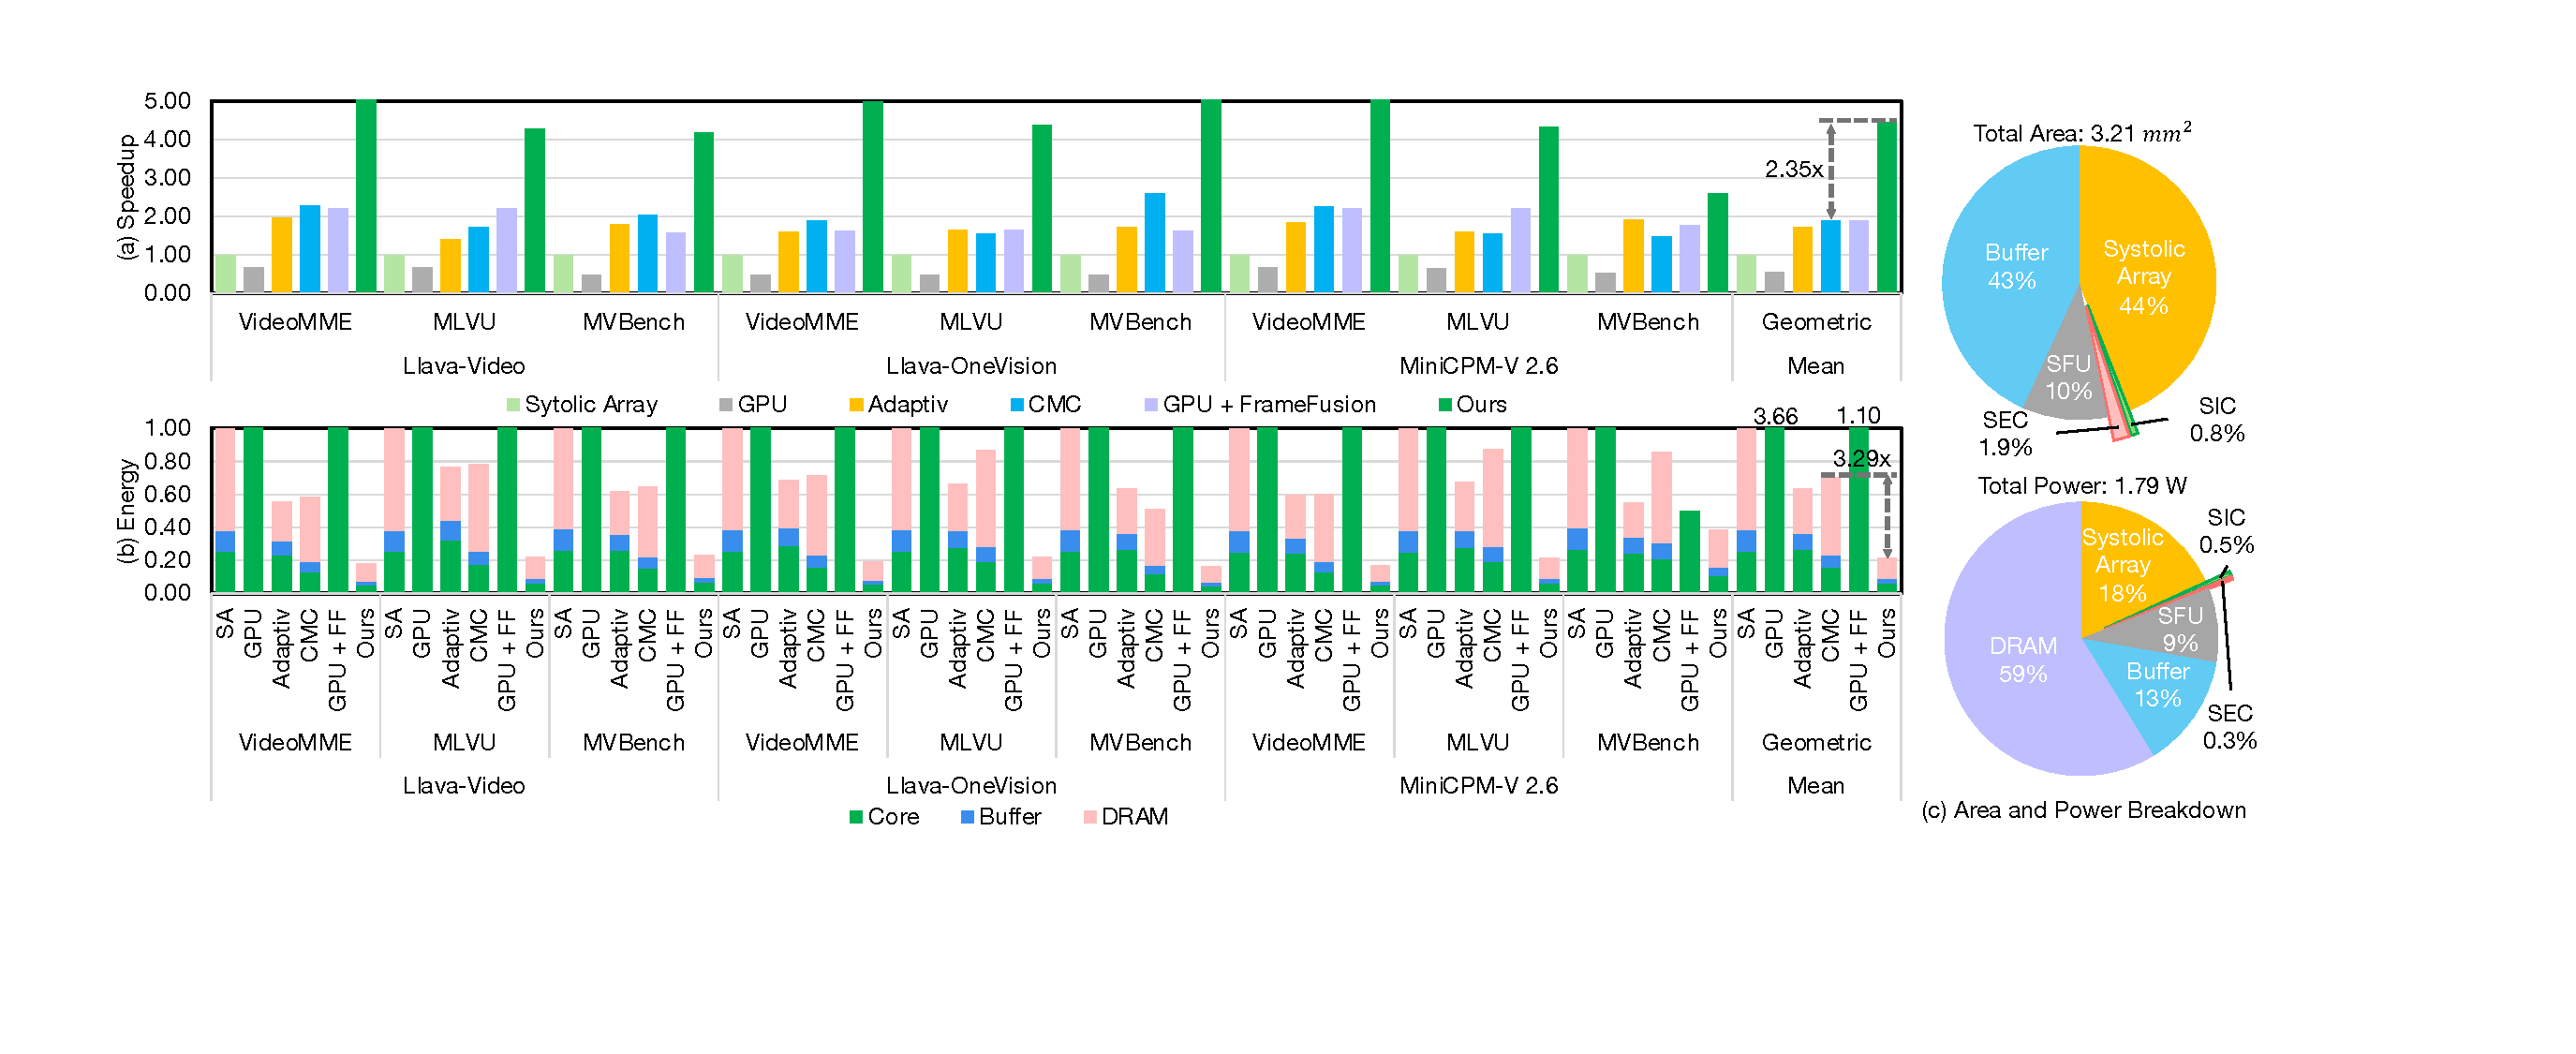
\includegraphics[width=1.0\linewidth]{figure/main.pdf}
    
    % \vspace{-1mm}
    \caption{{Left: Speedup and Energy efficiency.} Right: Area and power breakdown}
    \label{fig:main}
    % \vspace{-2mm}
\end{figure*}



\subsection{Performance and Energy Evaluation}

We compare \proj against baseline methods, including the vanilla systolic array (SA), Adaptiv, and CMC, across multiple VLM models and datasets. The architectural setup for all baselines and \proj is detailed in \Tbl{tab:setup_compare}. We maintain the same frequency, technology node, number of processing elements, operand bit width, and DRAM bandwidth across all designs. {We further compare against the performance on an NVIDIA Jetson Orin Nano GPU~\cite{nvidia_jetson_orin_nano_2023}, evaluated with and without the FrameFusion algorithm.} The performance and energy results are presented in \Fig{fig:main} (a) and (b).

\textbf{Performance.}  
\proj achieves significant performance improvements across all benchmarks. On average, it delivers a 4.47$\times$ speedup over the vanilla systolic array, which process dense input. This improvement stems from the ability of multi-level concentration to aggressively compress input tokens, getting 80.2\% sparsity. 

Compared to AdapTiV, \proj achieves a \textbf{2.60$\times$} average speedup. While AdapTiV effectively detects and prunes nearby redundant visual tokens, it operates at a coarser granularity. In contrast, \proj performs vector-wise similarity removal, enabling finer-grained redundancy elimination. 

Against CMC, \proj achieves a \textbf{2.35$\times$} speedup. While CMC leverages external video codecs to perform wide-range redundancy search, this approach is often inefficient due to a high rate of mismatches. In contrast, \proj efficiently identifies sufficient redundancy within localized blocks using its on-chip similarity matcher.

{Compared with the GPU, our design achieves a $7.90\times$ speedup over the GPU and a $2.37\times$ speedup over the GPU running with FrameFusion. This improvement stems from our architecture’s ability to achieve higher computational utilization than the GPU. Moreover, \proj attains higher sparsity than FrameFusion due to its finer-grained redundancy removal, which is difficult to exploit on GPU Tensor Cores. 
}

\textbf{Energy Efficiency.}
As shown in \Fig{fig:main}(b), we report the total energy consumption of \proj and baseline designs, normalized to the vanilla systolic array (SA). The energy breakdown includes three components: on-chip core, on-chip buffer, and off-chip memory.

Compared to SA, {GPU,} AdapTiV, CMC, and {GPU with FrameFusion}, \proj achieves average energy efficiency improvements of {\textbf{4.67$\times$}}, {\textbf{17.09$\times$}} {\textbf{2.98$\times$}}, {\textbf{3.29$\times$}}, and {\textbf{5.13$\times$}}, respectively. These results highlight that \proj delivers significant savings across both computation and memory under constrained on-chip budget. This efficiency gain stems from our architecture's ability to sparsify output of GEMM on-chip immediately after output tile generation, ensuring that all subsequent off-chip memory transactions operate on compressed data. A detailed analysis of memory access reduction is presented in \Sec{sec:mem_access}.


\begin{table}[t]
    \centering
    \caption{Configuration comparison of \proj and baseline architecture}
    \resizebox{0.5\textwidth}{!}{
    \begin{tabular}{l|c|c|c|c}
    \toprule
        Architecture & SystolicArray & Adaptiv & CMC & Ours \\ \midrule
        Technology & 28nm & 28nm & 28nm & 28nm \\ \midrule
        Frequency & 500MHz & 500MHz & 500MHz & 500MHz \\ \midrule
        \multirow{2}{*}{PE Array} & 32x32 & 16x64 & 32x32 & 32x32 \\ 
         & 16-bit & 16-bit & 16-bit & 16-bit \\ \midrule
        Buffer Size& 734KB & 768KB & 907KB & 734KB \\ \midrule
        DRAM Bandwidth & 64GB/s & 64GB/s & 64GB/s & 64GB/s \\ \midrule
        On-chip Area/$mm^2$ & {3.12} & {3.38} & {3.58} & {3.21} \\ \midrule
        On-chip Power/mW & {720} & {1176} & {832} & {736} \\ \bottomrule
    \end{tabular}
    }
    % \vspace{-6mm}
    \label{tab:setup_compare}
\end{table}


\textbf{Area and Power Analysis.}
The area and power consumption of \proj and the baselines are also summarized in \Tbl{tab:setup_compare}. The power statistics is derived on Llava-Video-7B with VideoMME dataset. Our \proj design occupies {3.21}\,mm\textsuperscript{2} of on-chip area and consumes {736}\,mW of power, both of which are lower than those of Adaptiv and CMC.

\proj is smaller than CMC, as the external video codec used by CMC incurs substantial hardware overhead. Compared to Adaptiv, which adopts a lightweight similarity detection mechanism, \proj remains more efficient due to its streaming SEC that operates on localized input. Despite its enhanced functionality, \proj introduces only a {\textbf{2.7\%}} increase in area and a {\textbf{0.9\%}} increase in power consumption relative to the systolic array architecture.
These results highlight the efficiency and low overhead of the \proj unit, which delivers significant performance benefits within a modest hardware budget.

To gain a deeper understanding of the overhead introduced by \proj, we present a detailed breakdown in \Fig{fig:main}(c). We observe that the proposed Semantic Concentrator and Similarity Concentrator are both highly lightweight, accounting for only 1.9\% and 0.8\% of the overall area, respectively. These two units also contribute negligibly to the overall power consumption. This demonstrates that SEC and SIC are well-suited for resource-constrained scenarios.

{
\textbf{Overall Insights.} 
Beyond speedup and energy gains, \proj{} establishes a new paradigm for redundancy-aware VLM acceleration through tight algorithm–hardware co-design. 
At the \textbf{token level}, it performs on-the-fly \textit{Top-$k$ detection} via streaming processing, handling sparsity in real time with minimal cost.  
At the \textbf{block level}, a \textit{block-wise sliding window} propagates local similarity using only on-chip resources, reducing memory and buffer demand.  
At the \textbf{vector level}, \proj{} applies \textit{vector-wise similarity pruning} with a \textit{gather–scatter} scheme to control fine-grained irregular access and fully exploit sparsity.  
Together, these techniques translate algorithmic sparsity into tangible performance gains with minor hardware complexity.
}

\begin{figure}
    \centering
    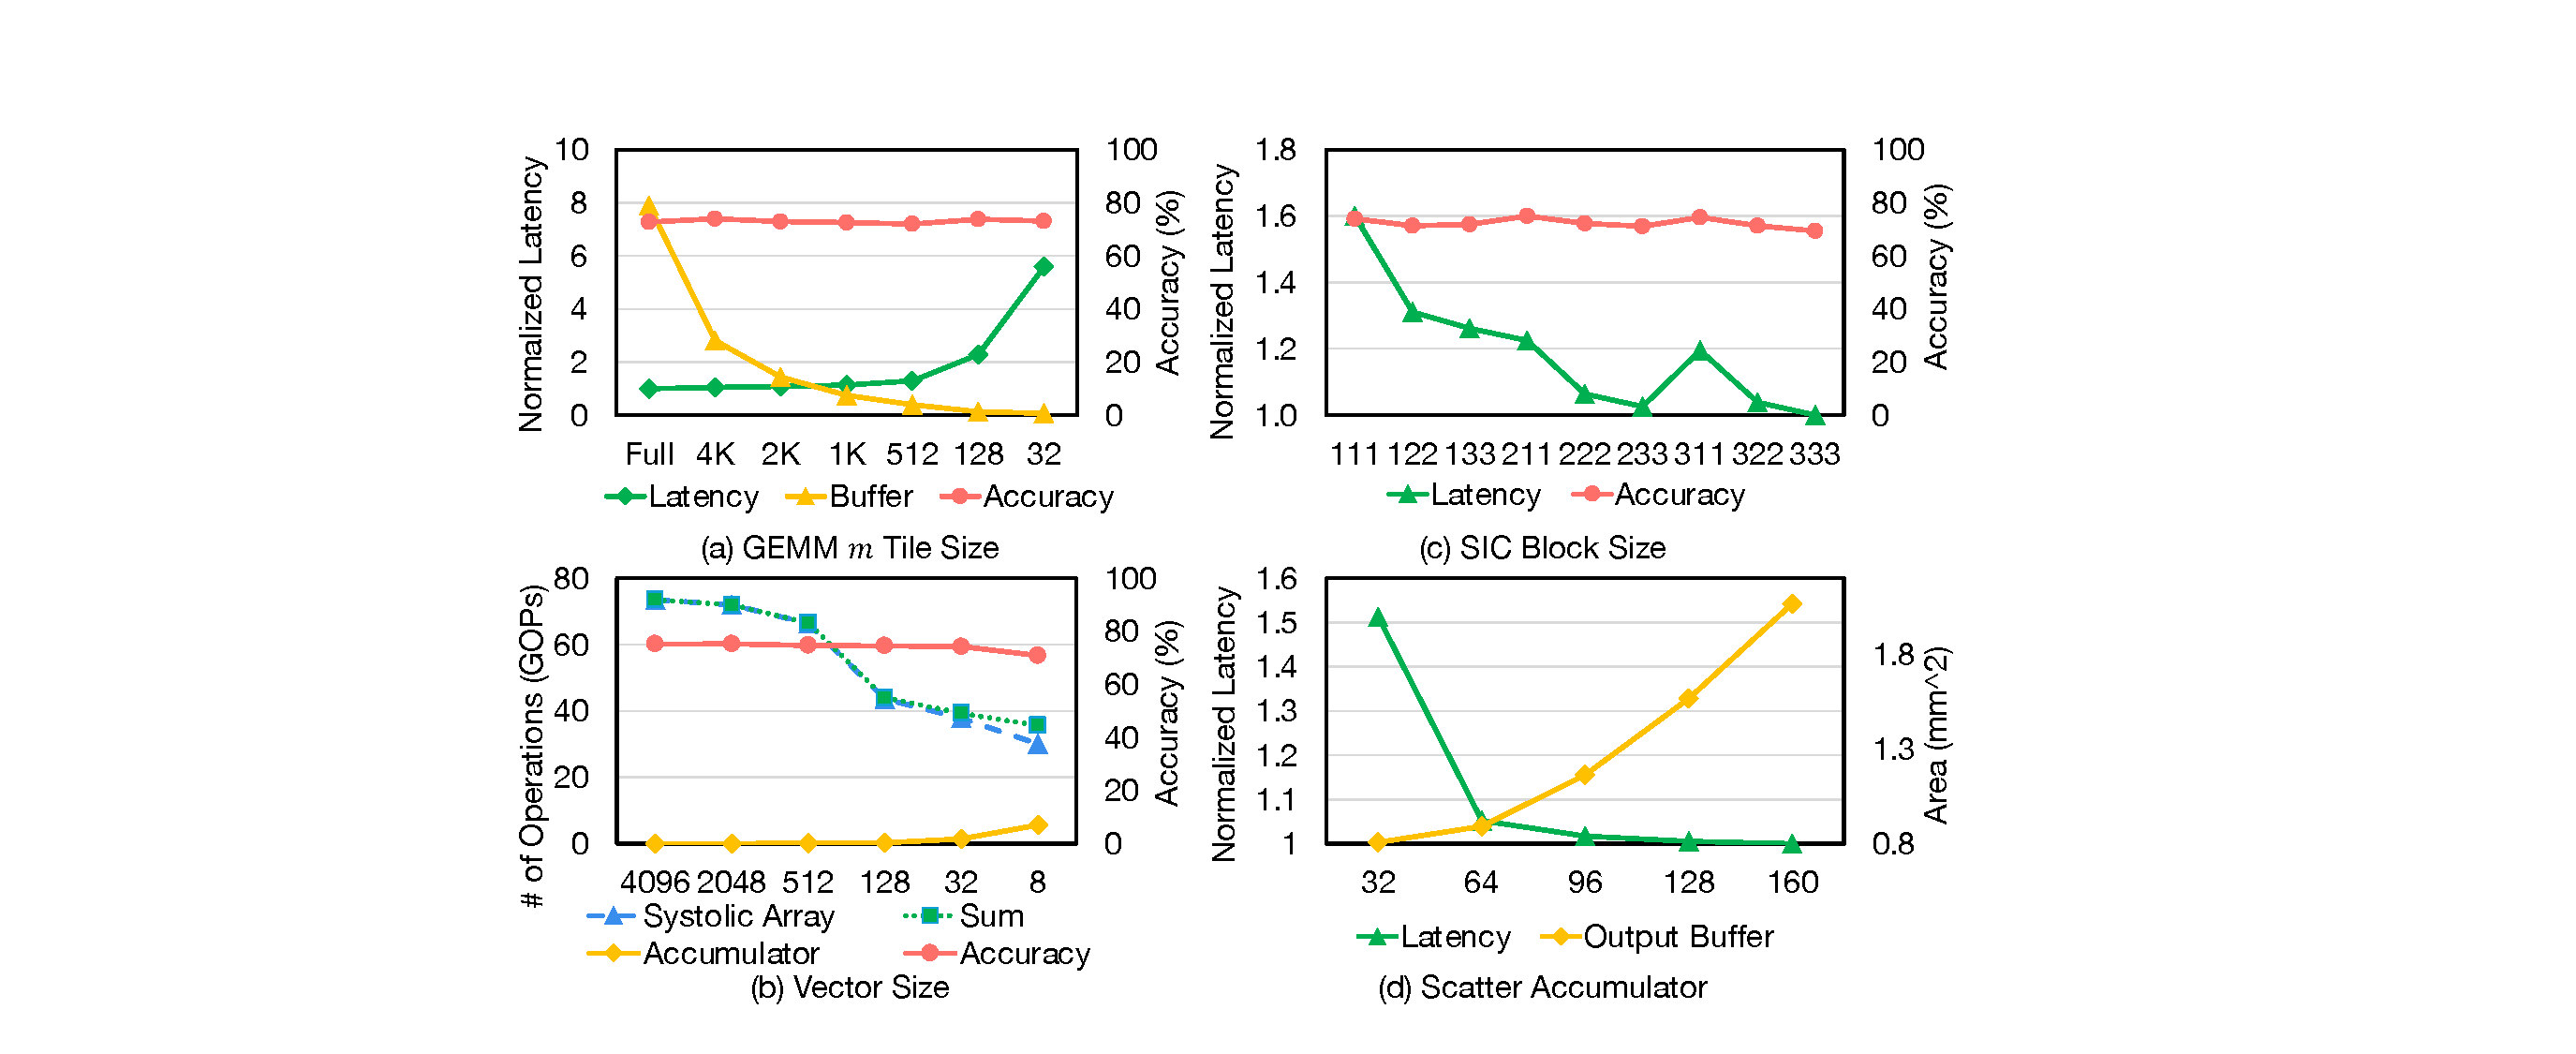
\includegraphics[width=1\linewidth]{figure/DSE.pdf}
    % \vspace{-5mm}
    \caption{{Design Space Exploration}}
    \label{fig:DSE}
    % \vspace{-5mm}
\end{figure}

\subsection{Design Space Exploration}

To evaluate the impact of key architectural parameters in \proj{}, we conduct a comprehensive design space exploration. We focus on four primary factors, varying each individually while fixing the others to their default values to isolate their effects. 
{Note that architectural parameters, other than the number of scatter accumulators, may also affect model accuracy. We evaluate accuracy under these variations and observe that the impact is generally negligible, allowing us to safely prioritize performance in our design exploration.}
All measurements are taken on the Llava-Video-7B model, using either the VideoMME or MLVU dataset.

\textbf{GEMM $m$ Tile Size.}
{As shown in \Fig{fig:DSE}(a), we sweep the tile size from the full input height down to 32. As the tile size decreases, the end-to-end latency steadily increases. {This trend arises because similarity gathering operates per tile. When a 2×2×2 block crosses tile boundaries, Focus only compares tokens within the same tile as the key token. For example, when the first token of a tile is the key, its neighbors outside the tile are unavailable for comparison. With smaller tile sizes (e.g., $m=32$), such boundary-crossing cases become more frequent, causing potentially similar vectors to be treated as distinct due to the limited comparison scope.}

While larger tiles offer better compression, they require more on-chip buffer to store intermediate results, increasing area and power consumption. We observe a trade-off between latency and buffer usage. From the latency–buffer curve in \Fig{fig:DSE}(a), a tile size of 1024 emerges as an optimal design point. It incurs only 19\% higher latency compared to the full-height tile while substantially reducing buffer requirements to a practical level.

\textbf{Vector Size.}
Vector size determines the granularity of similarity concentration and directly impacts the sparsity and operation counts. To assess this, we measure the number of operations of a layer in two main components of \proj{}: (1) MAC operations in the main systolic array, and (2) accumulation operations in the outer accumulator during Similarity Scatter.

As shown in \Fig{fig:DSE}(b), reducing the vector size leads to fewer operations in the systolic array. This is because smaller vectors enable finer-grained similarity comparisons, allowing more aggressive redundancy removal and reducing the input size to the PE array. However, smaller vector sizes also increase the number of K-dimension iterations, requiring more frequent accumulation, which in turn raises the operation count in the accumulator.

Beyond operation count, the systolic array dimension $b$ must be equal to or less than the vector size to utilize the benefits of fine-grained input. Taking both operational efficiency and hardware compatibility into account, we identify a vector size of 32 as an optimal design point, achieving strong compression while maintaining high utilization of the systolic array.

\begin{figure}[t]
    \centering
    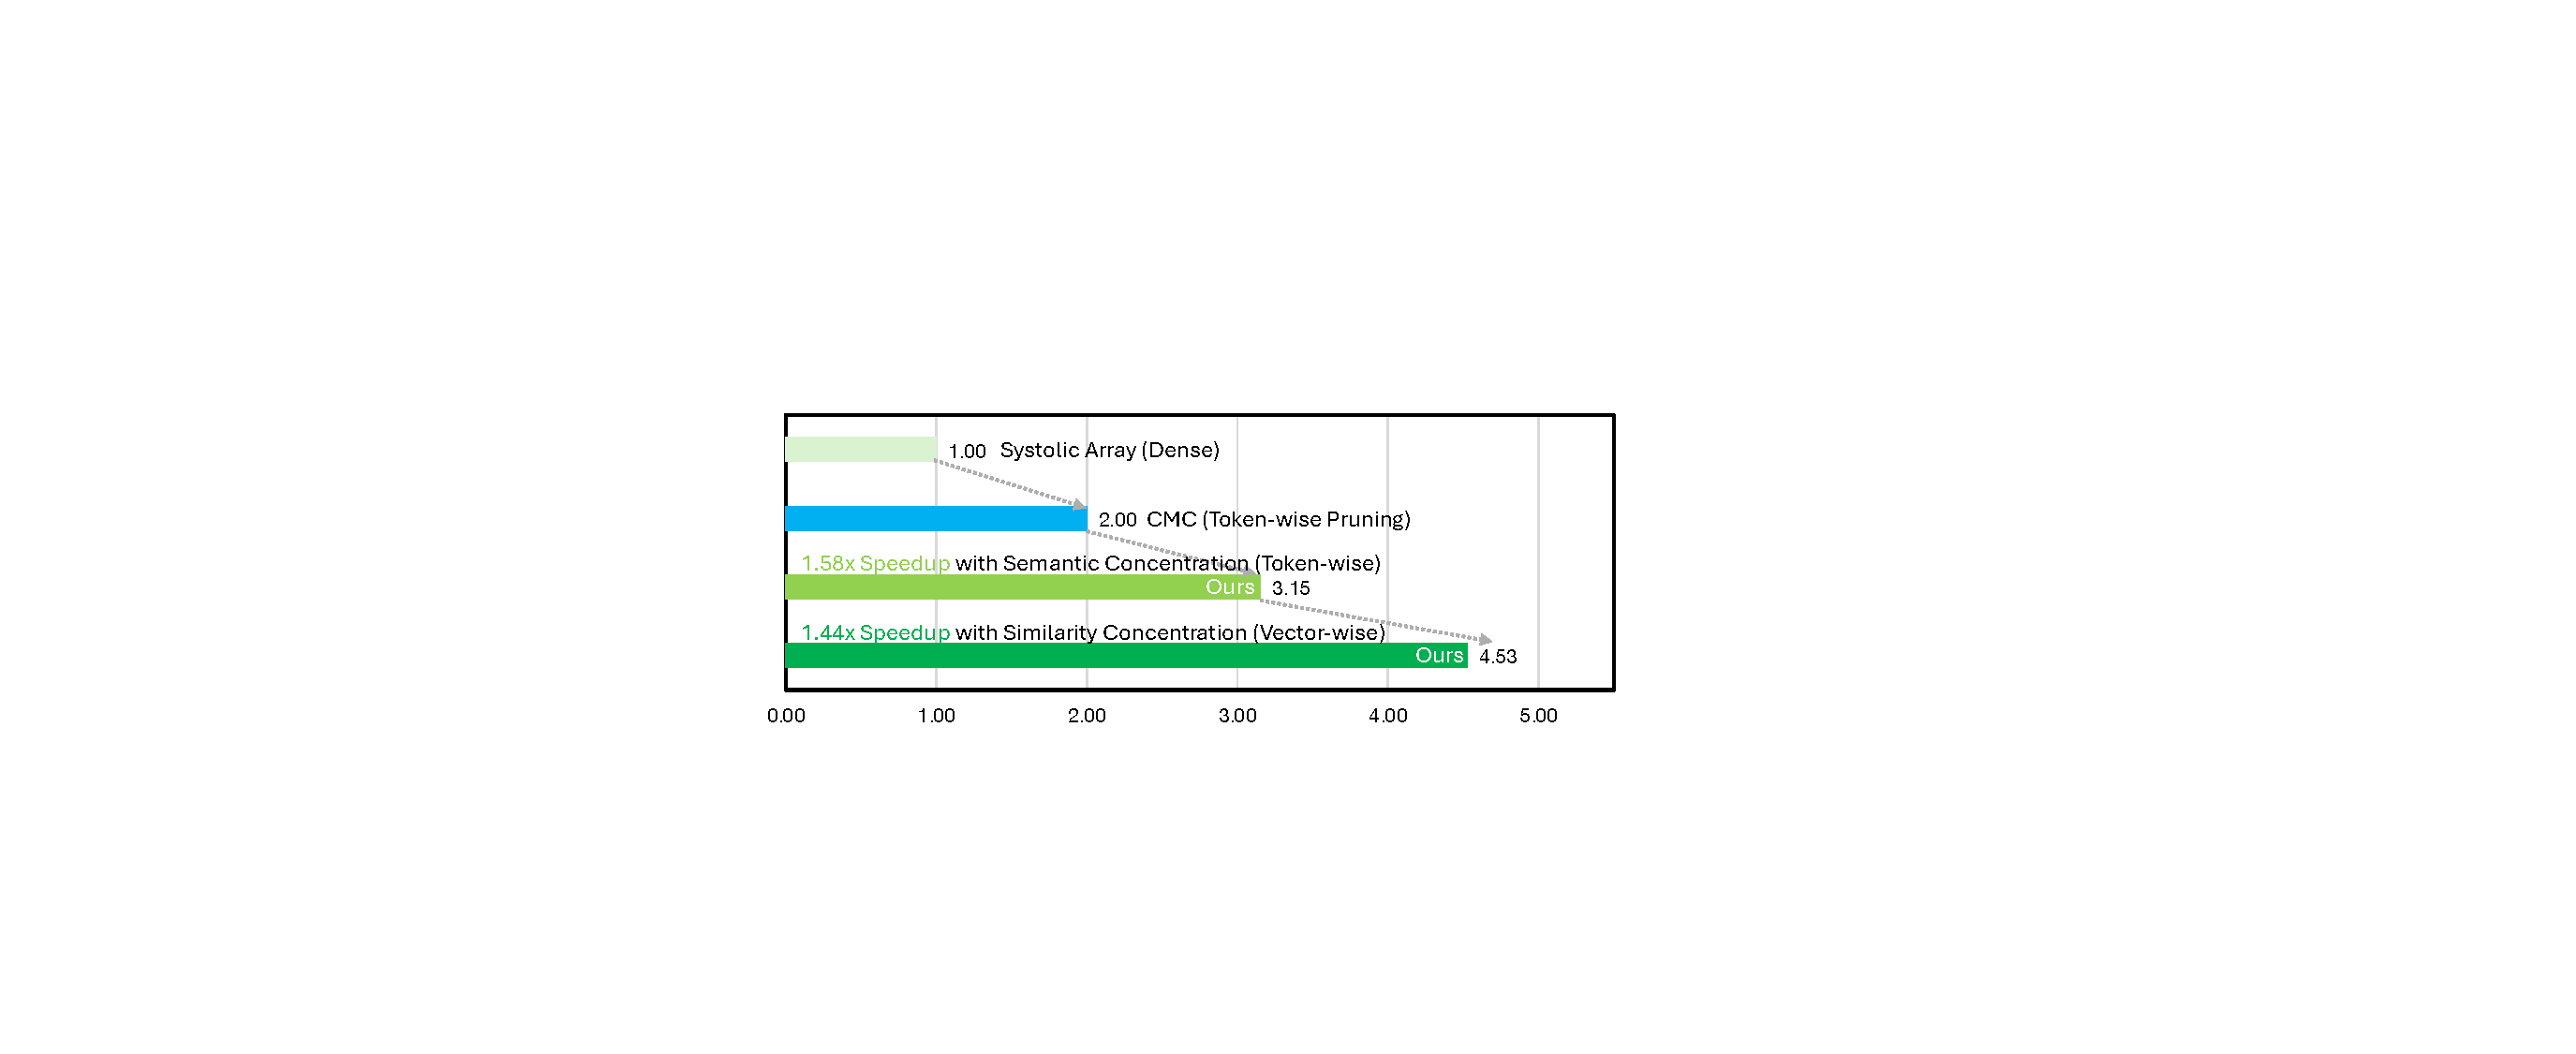
\includegraphics[width=0.99\linewidth]{figure/ablation.pdf}    
    % \vspace{-8mm}
    \caption{Ablation Study for \proj}
    \label{fig:ablation}    
    % \vspace{-5mm}
\end{figure}

\textbf{Similarity Concentrator Block Size.}
The block size used in the SIC directly impacts the spatial and temporal context available for similarity detection. 
{We vary the block size along both the temporal (frame) and spatial (height and width) dimensions to examine its impact on performance.}
{As shown in \Fig{fig:DSE}(c), the three-digit labels on the x-axis denote block sizes across these dimensions (e.g., 122 indicates f=1,h=2,w=2). We observe that enlarging the block size in either temporal or spatial dimensions reduces latency, as larger blocks provide broader context for similarity detection.}
{Notably, extending the block size along the temporal dimension yields a more pronounced latency reduction compared to spatial extensions, which we attribute to the strong inter-frame similarity inherent in video inputs.}
We find that a block size of 2×2×2 is sufficient to provide strong performance. 

\textbf{Scatter Accumulator.}
The number of accumulators in similarity scatter affects throughput and pipeline efficiency. Ideally, accumulation should finish before the next output tile arrives from the systolic array.
As shown in \Fig{fig:DSE}(d), using 64 accumulators achieves near-peak performance with only a 5\% latency overhead compared to a larger 160-accumulator design, with diminishing returns beyond that point. 
This configuration also simplifies buffer design.

{\textbf{Semantic Pruning Configuration.}
In our Semantic Pruning scheme, the value of “k” in top-k pruning is determined by multiplying the original number of image tokens by a predefined retention ratio. We search multiple layer-wise retention configurations and select the one offering the best sparsity–accuracy trade-off, which is adopted in our design. The final setup is summarized in \Tbl{tab:hardware-config}, where pruning is applied to five selected layers whose retention ratios differ from the preceding layer.
Future work may further enhance this strategy by dynamically adapting to input contexts, e.g., using a post-softmax attention threshold or top-p pruning~\cite{lin2025twilight}, though such adaptation can introduce runtime variations across inputs.
}

\subsection{Ablation Study}

{To assess the contribution of each component in \proj, we perform an ablation study on Llava-Video-7B and report speedup, as shown in \Fig{fig:ablation}. We incrementally enable the SEC and SIC, comparing results against a dense systolic baseline and CMC~\cite{song2024cmc}.
When only the SEC is enabled, \proj{} achieves a 3.15$\times$ speedup over the uncompressed systolic baseline and a \textbf{1.58$\times$} speedup over CMC. This demonstrates that semantic-aware pruning remove a large fraction of irrelevant visual tokens based on textual guidance, outperforming prior token-pruning strategies.

Enabling the vector-wise SIC further boosts speedup by an additional \textbf{1.44$\times$}. This highlights the ability of SIC to exploit residual redundancy among retained tokens at a finer vector granularity, beyond what semantic pruning alone can uncover.
SEC and SIC together yield a 4.53$\times$ speedup over the dense baseline and 2.26$\times$ over CMC, confirming the effectiveness and efficiency of the \proj{} design.}

\begin{figure}
    \centering
    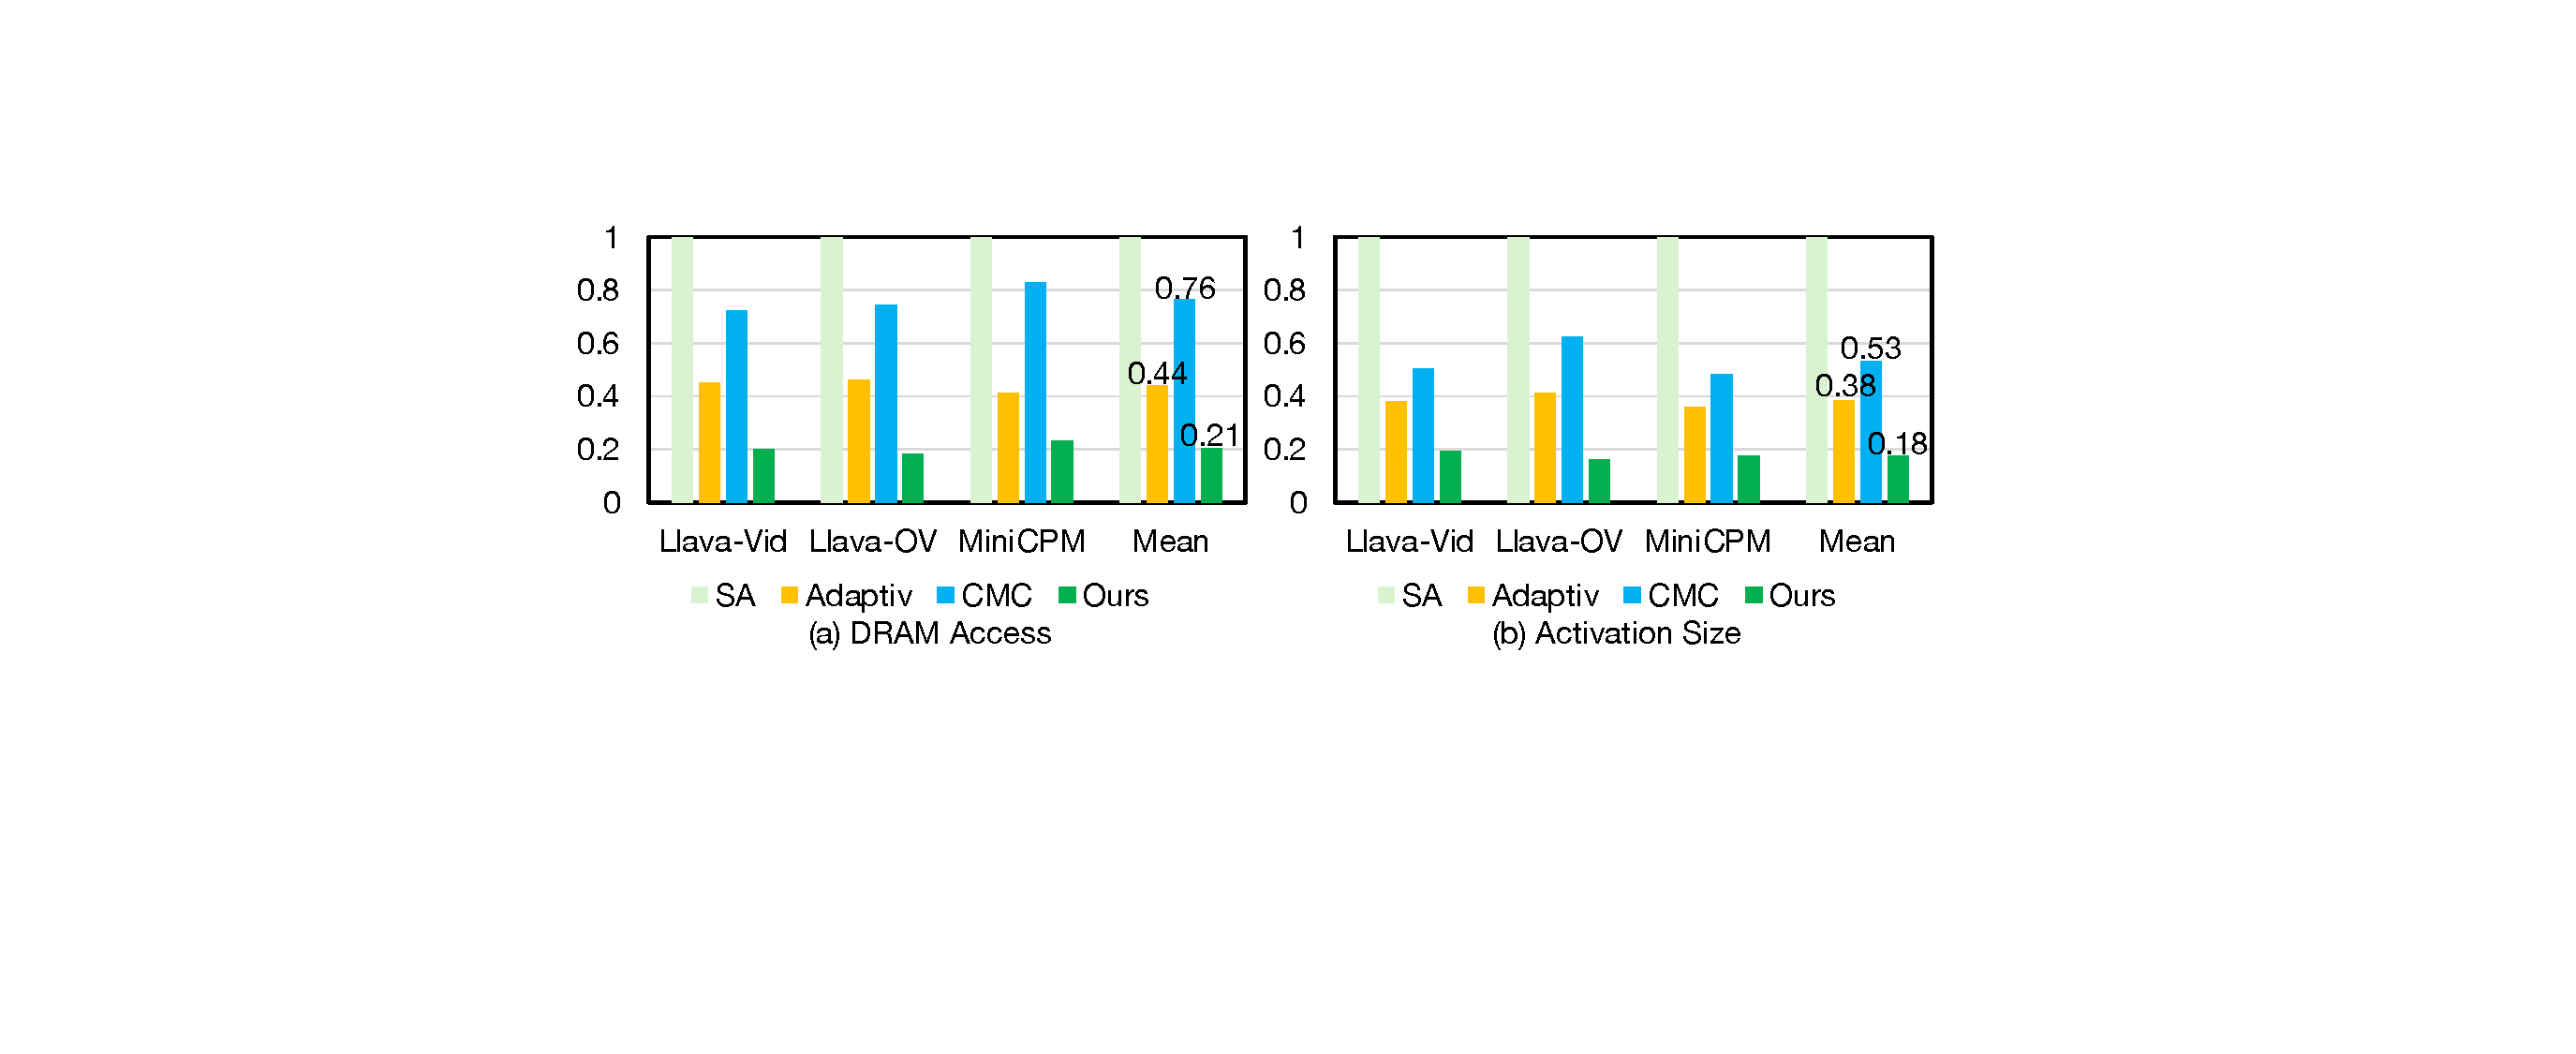
\includegraphics[width=\linewidth]{figure/mem_access.pdf}    
    % \vspace{-6mm}
    \caption{Memory access analysis (a) overall DRAM access (b) activation size}
    \label{fig:mem_access}    
    % \vspace{-4mm}
\end{figure}

\subsection{Memory Access}
\label{sec:mem_access}

We analyze the off-chip memory traffic and {average} input matrix size of \proj{} compared to baseline designs. As shown in \Fig{fig:mem_access}(a) and (b), \proj{} achieves the lowest DRAM access and input matrix size across all methods. Compared to the dense systolic array, we compress the input matrix by 5.6$\times$ and reduce memory traffic by 4.9$\times$.

This reduction stems from the joint effect of the SEC and SIC, which sparsifies the input at both token and vector levels. Additionally, the output of each FC layer is immediately compressed on-chip before being written to memory, so only compressed activations are transferred to DRAM, minimizing total memory access.

Compared to both CMC and AdapTiV, \proj{} achieves significantly higher input compression and lower DRAM access: \textbf{3.0$\times$} and \textbf{2.2$\times$} higher compression ratios, and \textbf{3.7$\times$} and \textbf{2.2$\times$} DRAM traffic reduction, respectively. 

CMC relies on codec-based similarity detection over wide temporal windows and full-token representations, requiring large uncompressed regions to be staged in DRAM before processing. This leads to redundant memory transfers, as data must be written and read again for similarity detection. Similarly, AdapTiV performs local token pruning but still processes on whole-token granularity.
By avoiding these limitations through lightweight, streaming-compatible similarity matching, \proj{} achieves superior memory efficiency with minimal overhead.

\subsection{Synergy with Quantization}
{\proj is fully compatible with standard quantization techniques. We integrate \proj{} with INT8 quantization using bitsandbytes~\cite{dettmers20218}, and the results in \Tbl{tab:int8_degrade} show the impact on accuracy and sparsity compared to FP16. INT8 causes an average accuracy drop of 0.5\% and a sparsity change of 0.13\% relative to FP16. Although this loss is slightly higher than the 0.02\% degradation in the dense model, it is reasonable since \proj and quantization jointly compress the model. Overall, the accuracy drop remains minor, and \proj effectively maintains its redundancy-removal capability under quantization, demonstrating strong synergy for efficient VLM inference.}

\begin{table}[t]
    \centering
    \caption{{Influence of INT8 quantization on accuracy and sparsity}}
    % \vspace{-2mm}
    \resizebox{0.48\textwidth}{!}{
    \begin{tabular}{l|l|c|c|c|c|c|c}
    \toprule
        \multirow{2}{*}{Models} & \multirow{2}{*}{Datasets} 
        & \multicolumn{2}{c|}{Dense} 
        & \multicolumn{2}{c|}{Ours} 
        & \multicolumn{2}{c}{Ours} \\ 
        \cmidrule{3-8}
        ~ & ~ & Acc. & Degrade & Acc. & Degrade & Sparsity & Degrade \\ 
    \midrule
        \multirow{3}{*}{Llava-Vid} 
        & VMME & 64.22 & -0.07 & 62.33 & 0.41 & 82.48 & 0.34 \\ 
        & MLVU & 68.21 & -0.47 & 64.94 & 1.05 & 78.10 & 0.17 \\ 
        & MVB  & 59.75 &  0.58 & 57.95 & 0.25 & 78.04 & 0.40 \\ 
    \midrule
        \multirow{3}{*}{Llava-OV} 
        & VMME & 58.70 & -0.29 & 57.44 & 1.26 & 81.46 & 0.03 \\ 
        & MLVU & 63.38 & -0.06 & 62.41 & 0.11 & 78.35 & -0.01 \\ 
        & MVB  & 58.55 & -0.17 & 56.18 & 0.60 & 85.35 & 0.14 \\ 
    \midrule
        \multirow{3}{*}{MiniCPM} 
        & VMME & 58.63 &  0.18 & 57.96 & 0.34 & 82.84 & 0.03 \\ 
        & MLVU & 55.93 & -0.04 & 53.22 & 0.37 & 77.99 & 0.02 \\ 
        & MVB  & 55.13 &  0.50 & 54.03 & 0.27 & 75.97 & 0.02 \\ 
    \bottomrule
    \end{tabular}
    \label{tab:int8_degrade}
    }
    % \vspace{-4mm}
\end{table}



\section{Discussion}
\label{sec:disc}


\subsection{Generalization Ability of \proj}
{We further examine the generalization ability of \proj. Although \textit{Focus} is originally designed for video-based VLMs, it can be directly extended to image-based VLMs by treating a single image as a one-frame video. While temporal similarity is no longer present in this setting, substantial semantic redundancy and spatial similarity remain. As shown in \Tbl{tab:image}, evaluations on image-based VLMs~\cite{li2024llava,bai2025qwen2} across multiple datasets~\cite{goyal2017making,liu2024mmbench,zhang2021mme} demonstrate notable speedups over both the systolic-array baseline and AdapTiV, with only minor accuracy degradation. These results indicate that \proj effectively removes redundancy beyond the video domain.}

Moreover, \proj can potentially be extended to Vision--Language--Action (VLA)~\cite{kim2024openvla,intelligence2504pi0} models for embodied AI applications. VLA models share similar input modalities with VLMs, including image or video inputs paired with text. Therefore, we believe the SEC and SIC in \proj could effectively eliminate redundant information in VLA inputs, making this a promising direction for future exploration.


\begin{table}[t]
    \centering
    \caption{Accuracy and Speedup on image VLMs}
    % \vspace{-2mm}
    \resizebox{0.47\textwidth}{!}{
    \begin{tabular}{l|l|l|c|c|c}
    \toprule
        Models & Dataset & Metric & Dense & AdapTiV & Ours \\ \midrule
        \multirow{6}{*}{Llava-OneVision} 
        & \multirow{2}{*}{VQAv2} & Speedup & 1.00 & \textbf{5.19} & 4.44 \\ 
        & ~ & Accuracy & 84.32 & 82.48 & \textbf{83.01} \\ \cmidrule{2-6}
        & \multirow{2}{*}{MME} & Speedup & 1.00 & 1.65 & \textbf{4.26} \\ 
        & ~ & Score & 1067.27 & 1036.27 & \textbf{1044.79}  \\ \cmidrule{2-6}
        & \multirow{2}{*}{MMBench} & Speedup & 1.00 & 1.60 & \textbf{4.25} \\ 
        & ~ & Accuracy & 84.99 & \textbf{84.49} & 83.46 \\ \midrule
        \multirow{6}{*}{Qwen2.5-VL} 
        & \multirow{2}{*}{VQAv2} & Speedup & 1.00 & \textbf{1.96} & 1.91 \\ 
        & ~ & Accuracy & 84.48 & 79.77 & \textbf{81.73} \\ \cmidrule{2-6}
        & \multirow{2}{*}{MME} & Speedup & 1.00 & 1.89 & \textbf{1.97} \\ 
        & ~ & Score & 1337.66 & 1129.56 & \textbf{1238.88} \\ \cmidrule{2-6}
        & \multirow{2}{*}{MMBench} & Speedup & 1.00 & \textbf{1.93} & 1.78 \\ 
        & ~ & Accuracy & 85.69 & 83.79 & \textbf{84.46} \\
    \bottomrule
    \end{tabular}
    \label{tab:image}
    }    
% \vspace{-2mm}
\end{table}

\subsection{Worst- and Best-Case Analysis}
{Since sparsity varies with video content, we analyze two extreme scenarios to verify robustness.} {In the \textbf{worst case}, when no similarity exists across frames or patches, sparsity drops near zero. The design preserves the full tile length ($m=1024$), with buffers sized for maximum data without overflow.} {In the \textbf{best case}, abundant similarity yields highly compressed tiles and small $m$, slightly wasting buffer space and underutilizing the systolic array but remaining correct.} {We further aggregate the frequency of different tile lengths (i.e. number of vectors) and measure systolic-array utilization (\Fig{fig:worst_case}). These extremes are rare, one increases latency, the other lowers utilization, but the system maintains an average utilization of 92.2\%, confirming robust performance across diverse inputs.
}


\subsection{Related Works}

\textbf{Algorithm Optimizations.} 
As a major paradigm for multimodal reasoning, VLMs have attracted significant attention, resulting in a rapidly growing body of work on improving inference efficiency. 
A large class of recent methods focuses on exploiting redundancy in visual tokens to accelerate VLM inference~\cite{fu2024framefusion,fastv,huang2025prunevid,shen2025fastvid,liu2025keyframe,wang2025corematching,liu2025nvila}. 
FrameFusion~\cite{fu2024framefusion} compares and merges similar tokens across adjacent frames, while PruneVid~\cite{huang2025prunevid} performs token clustering and merges tokens within the same cluster. 
By removing or compressing redundant tokens through diverse algorithmic strategies, these approaches effectively reduce token counts and achieve notable speedups on GPUs.

Despite their effectiveness, these methods operate exclusively at the token level and are implemented as software-only optimizations. 
They are primarily designed for execution on general-purpose GPUs and do not consider how redundancy manifests at finer granularities or how it can be efficiently exploited from a bottom-up hardware perspective.


\begin{figure}[t]
    \centering
    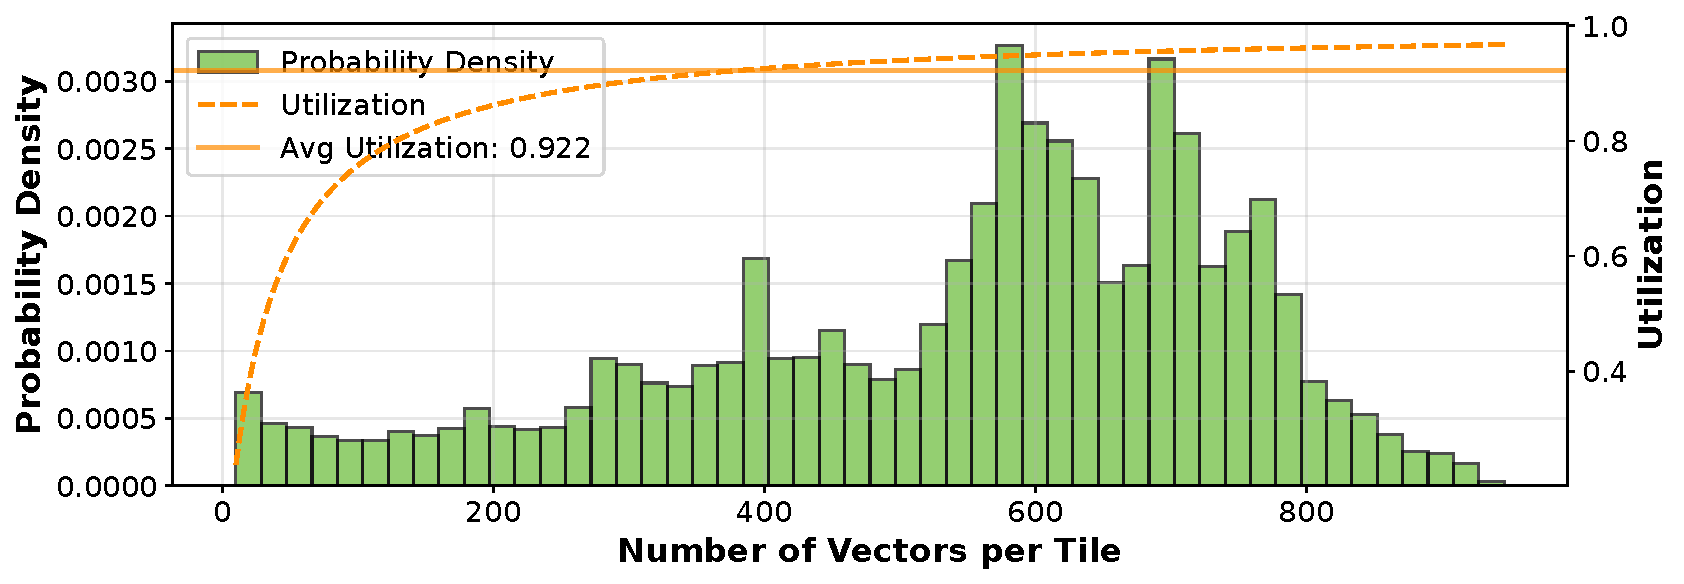
\includegraphics[width=\linewidth]{figure/worst_case.pdf}    
    % \vspace{-6mm}
    \caption{{Histogram and compute utilization of concentrated tile length.} }
    \label{fig:worst_case}    
    \vspace{-2mm}
\end{figure}

\textbf{Architecture Design.} 
From the hardware architecture perspective, to the best of our knowledge, there is no dedicated accelerator specifically designed for VLM inference. 
Existing architectural efforts instead target efficiency optimizations for LLMs and ViTs, which share the transformer backbone with VLMs. 
These works predominantly rely on sparsity~\cite{wang2021spatten,dong2023heatvit,you2023vitcod,wang2025lad,guo2020accelerating,wei2025prosperity,wei2025phi} and quantization~\cite{guo2023olive,chen2025bitmod,guo2022ant,hu2025m,cheng2025ecco,guo2025transitive}.
In terms of sparsity, SpAtten~\cite{wang2021spatten} introduces token- and head-level pruning for transformers, while LAD~\cite{wang2025lad} optimizes key--value cache pruning during the decoding phase of LLMs. 
HeatViT~\cite{dong2023heatvit} leverages attention maps in ViTs to prune visual tokens. 
In addition, several works propose hardware-friendly quantization architectures: Olive~\cite{guo2023olive} introduces an outlier--victim pair format integrated into processing element (PE) arrays, and BitMoD~\cite{chen2025bitmod} enables fine-grained data-type adaptation through bit-serial processing.

While these techniques can be applied to VLMs, they are not explicitly designed for multimodal workloads and therefore may fail to fully capture the unique redundancy patterns introduced by cross-modal interactions. 
In contrast, \proj is the first architecture specifically tailored for VLM inference. 
By exploiting cross-modal semantic redundancy and detecting fine-grained vector-level similarity, \proj enables efficient streaming execution and achieves superior hardware efficiency beyond token-level or modality-agnostic optimizations.
